\chapter{Acoustic measurements}

\Cref{fig:period_1k} shows a periodogram of the recorded audio signal with a 1kHz input on X2. The amplitude is the energy of the signal and the x-axis shows the frequency.
\begin{figure}[H]
    \centering
    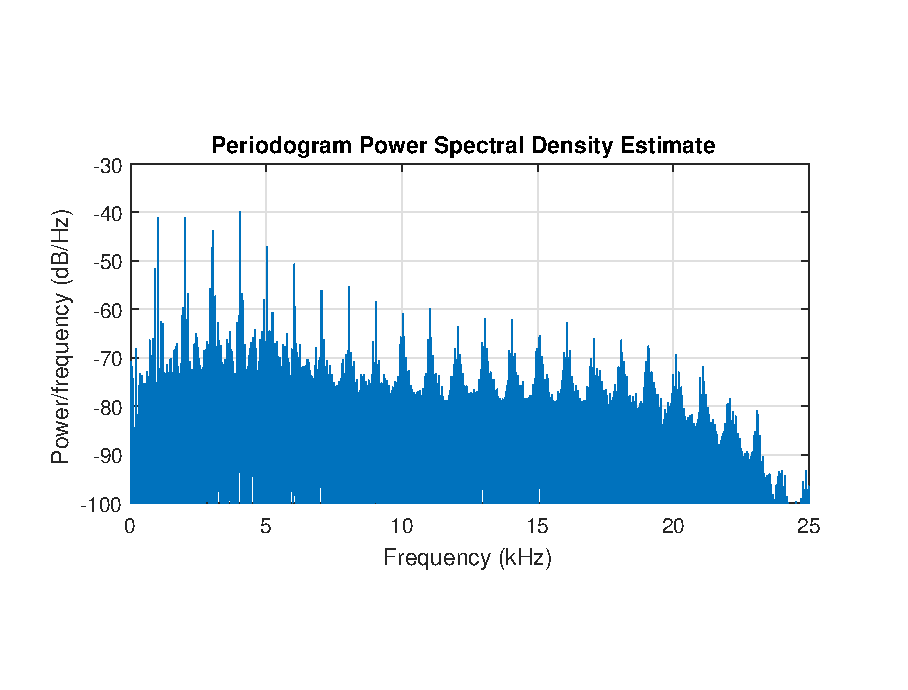
\includegraphics[trim={0cm 1.6cm 0cm 2cm},clip,width=\textwidth]{img/Periodogram_1khz-09.eps}
    \caption{Periodogram of 1kHz recorded tone}
    \label{fig:period_1k}
\end{figure}

Here we see the base frequency 1kHz and harmonics spaced 1kHz apart all the way through the range of human hearing. We see that the lowest three harmonics together with the base frequency are dominant, then the energy of the harmonics start to decrease. This implies the waveform rises sharply and has a short duration, which is consistent with a series of electrical discharges. The amplitudes of the harmonics are shown in \cref{tab:1k_amps}.

\Cref{fig:recorded_1k} shows the waveform of the recorded audio signal with a 1kHz input on X2.

\begin{figure}[H]
    \centering
    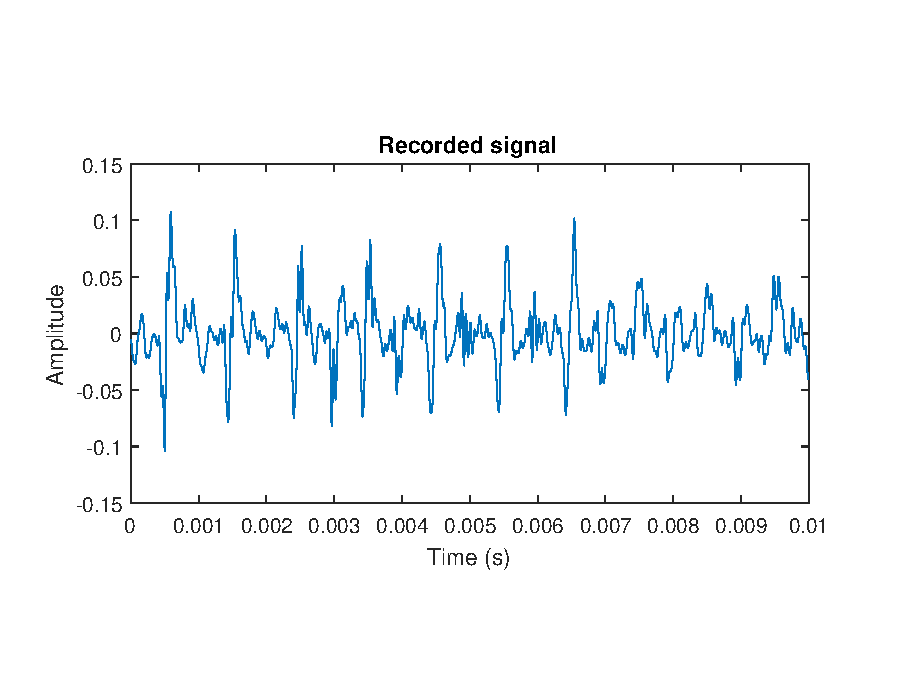
\includegraphics[trim={0cm 1.6cm 0cm 2cm},clip,width=\textwidth]{img/Recorded_1khz-09.eps}
    \caption{Time domain plot of 1kHz recorded tone}
    \label{fig:recorded_1k}
\end{figure}